\documentclass[tikz,border=12pt]{standalone}
\usepackage[T1]{fontenc}
\usepackage{lmodern}
\usetikzlibrary{arrows.meta,positioning,calc,backgrounds}
\definecolor{ink}{HTML}{20343B}
\definecolor{teal}{HTML}{2B6864}
\definecolor{mist}{HTML}{EFF6F4}
\definecolor{violet}{HTML}{665474}
\definecolor{wash}{HTML}{F5F2F7}
\begin{document}
\hyphenpenalty=10000
\exhyphenpenalty=10000
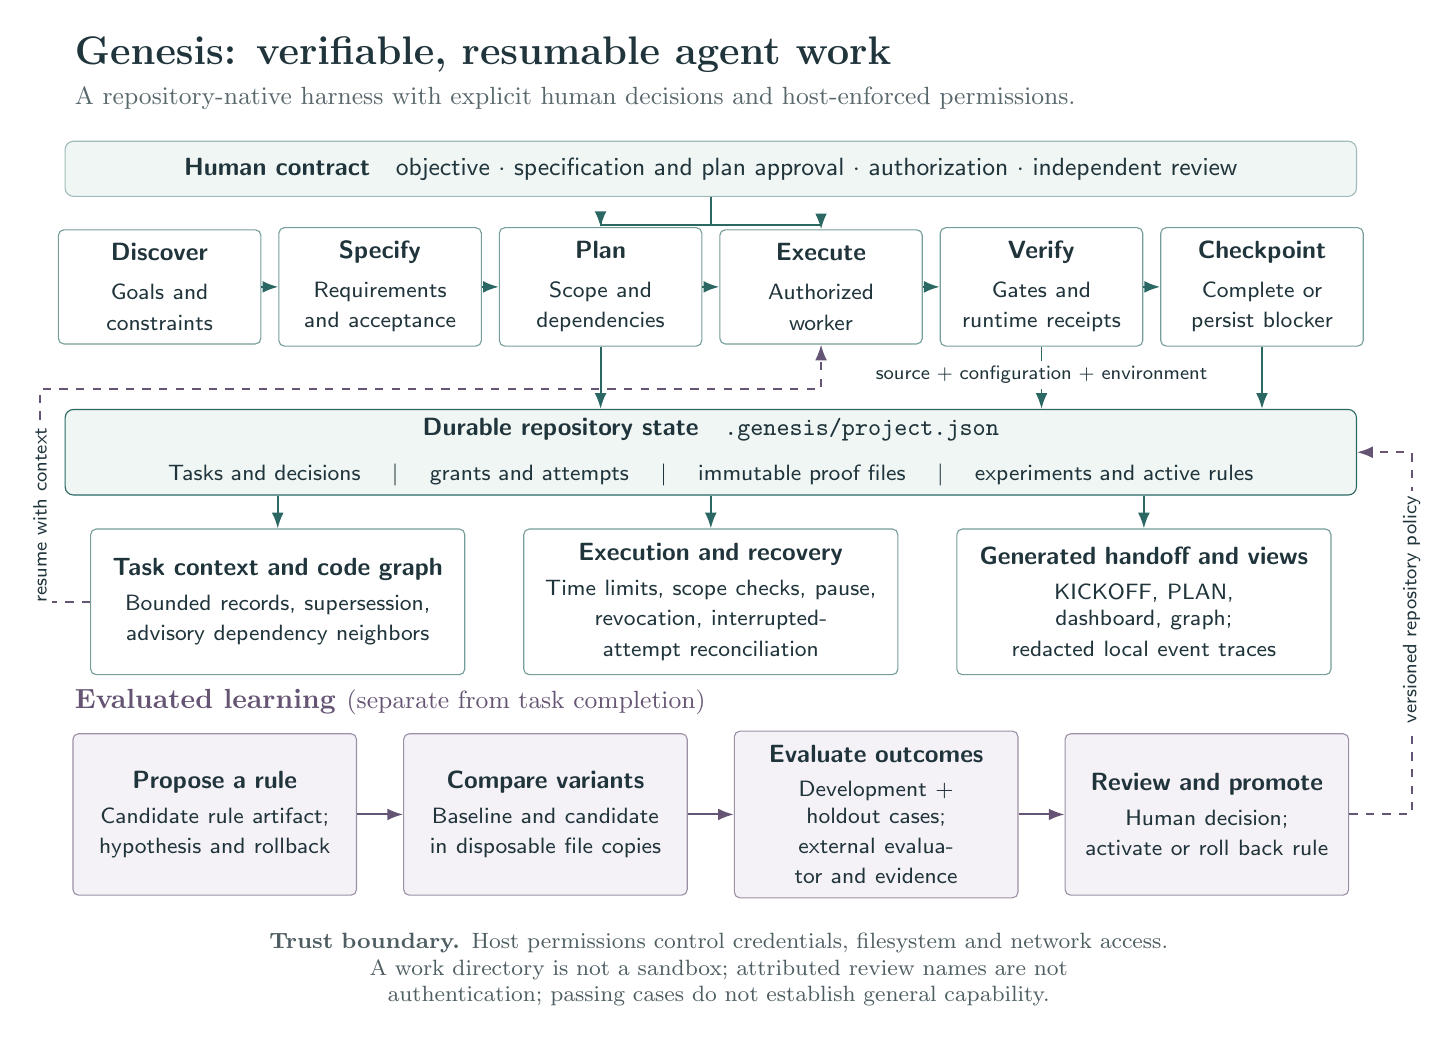
\begin{tikzpicture}[
  font=\sffamily\small, text=ink,
  box/.style={draw=teal!65,fill=white,rounded corners=2pt,align=center,minimum height=1.12cm,text width=2.22cm,inner sep=5pt},
  wide/.style={box,text width=4.4cm,minimum height=1.85cm},
  flow/.style={-{Latex[length=2mm]},draw=teal,line width=.7pt},
  feedback/.style={flow,dashed,draw=violet},
  label/.style={font=\sffamily\scriptsize,fill=white,inner sep=2pt},
]
\node[font=\rmfamily\Large\bfseries,anchor=west] at (-.25,10.9) {Genesis: verifiable, resumable agent work};
\node[font=\rmfamily\small,anchor=west,text=ink!75] at (-.25,10.35) {A repository-native harness with explicit human decisions and host-enforced permissions.};

\node[draw=teal!45,fill=mist,rounded corners=3pt,minimum width=16.4cm,minimum height=.7cm] (human) at (7.95,9.45) {\textbf{Human contract}\quad objective $\cdot$ specification and plan approval $\cdot$ authorization $\cdot$ independent review};

\foreach \x/\id/\title/\detail in {
0.95/discover/Discover/Goals and constraints,
3.75/spec/Specify/Requirements and acceptance,
6.55/plan/Plan/Scope and dependencies,
9.35/work/Execute/Authorized worker,
12.15/proof/Verify/Gates and runtime receipts,
14.95/checkpoint/Checkpoint/Complete or persist blocker}
  \node[box] (\id) at (\x,7.95) {\textbf{\title}\\[3pt]\footnotesize \detail};
\foreach \a/\b in {discover/spec,spec/plan,plan/work,work/proof,proof/checkpoint}
  \draw[flow] (\a) -- (\b);
\draw[flow] (human.south) -- ++(0,-.36) -| (plan.north);
\draw[flow] (human.south) -- ++(0,-.36) -| (work.north);

\node[draw=teal,fill=mist,rounded corners=3pt,align=center,minimum width=16.4cm,minimum height=1.03cm] (spine) at (7.95,5.85) {
\textbf{Durable repository state}\quad \texttt{.genesis/project.json}\\[5pt]
\footnotesize Tasks and decisions $\quad\vert\quad$ grants and attempts $\quad\vert\quad$ immutable proof files $\quad\vert\quad$ experiments and active rules};
\draw[flow] (plan.south) -- (plan.south |- spine.north);
\draw[flow] (proof.south) -- (proof.south |- spine.north);
\draw[flow] (checkpoint.south) -- (checkpoint.south |- spine.north);
\node[label] at (12.15,6.83) {source + configuration + environment};

\node[wide] (context) at (2.45,3.95) {\textbf{Task context and code graph}\\[3pt]\footnotesize Bounded records, supersession,\\advisory dependency neighbors};
\node[wide] (recovery) at (7.95,3.95) {\textbf{Execution and recovery}\\[3pt]\footnotesize Time limits, scope checks, pause,\\revocation, interrupted-attempt reconciliation};
\node[wide] (views) at (13.45,3.95) {\textbf{Generated handoff and views}\\[3pt]\footnotesize KICKOFF, PLAN, dashboard, graph;\\redacted local event traces};
\foreach \n in {context,recovery,views}
  \draw[flow] (spine.south -| \n.north) -- (\n.north);
\draw[feedback] (context.west) -- (-.57,3.95) -- (-.57,6.65) -| (work.south);
\node[label,rotate=90] at (-.57,5.05) {resume with context};

\node[font=\rmfamily\normalsize\bfseries,anchor=west,text=violet] at (-.25,2.68) {Evaluated learning \textnormal{\small (separate from task completion)}};
\node[box,draw=violet!65,fill=wash,text width=3.25cm,minimum height=2.05cm] (proposal) at (1.65,1.25) {\textbf{Propose a rule}\\[3pt]\footnotesize Candidate rule artifact;\\hypothesis and rollback};
\node[box,draw=violet!65,fill=wash,text width=3.25cm,minimum height=2.05cm] (compare) at (5.85,1.25) {\textbf{Compare variants}\\[3pt]\footnotesize Baseline and candidate\\in disposable file copies};
\node[box,draw=violet!65,fill=wash,text width=3.25cm,minimum height=2.05cm] (evaluate) at (10.05,1.25) {\textbf{Evaluate outcomes}\\[3pt]\footnotesize Development + holdout cases;\\external evaluator and evidence};
\node[box,draw=violet!65,fill=wash,text width=3.25cm,minimum height=2.05cm] (promote) at (14.25,1.25) {\textbf{Review and promote}\\[3pt]\footnotesize Human decision;\\activate or roll back rule};
\foreach \a/\b in {proposal/compare,compare/evaluate,evaluate/promote}
  \draw[flow,draw=violet] (\a) -- (\b);
\draw[feedback] (promote.east) -- (16.85,1.25) -- (16.85,5.85) -- (spine.east);
\node[label,rotate=90] at (16.85,3.85) {versioned repository policy};

\node[align=center,text width=16.7cm,font=\rmfamily\footnotesize,text=ink!80] at (8.05,-.72) {
\textbf{Trust boundary.} Host permissions control credentials, filesystem and network access.\\
A work directory is not a sandbox; attributed review names are not authentication; passing cases do not establish general capability.};
\end{tikzpicture}
\end{document}
